\documentclass{paper}
\usepackage{nomencl}
\usepackage{amsmath}
\usepackage{graphicx}
\usepackage{parskip}
\usepackage{hyperref}
\usepackage[toc,page]{appendix}
\usepackage{subcaption}
\usepackage{csquotes}
\usepackage{framed}
\usepackage{amsthm}
\usepackage{xcolor}

\newtheoremstyle{own}%
    {3pt}% Space above
    {3pt}% Space below
    {}% Body font
    {}% Indent amount
    {\color{blue}\bfseries}% Theorem head font
    {:}% Punctuation after theorem head
    {\newline}% Space after theorem head
    {}% Theorem head spec

\theoremstyle{definition}
\newtheorem{exmp}{Example}[section]

\theoremstyle{theorem}
\newtheorem{theorem}{Theorem}[section]
 
\theoremstyle{definition}
\newtheorem{definition}{Definition}[section]

\theoremstyle{remark}
\newtheorem{remark}{Remark}[section]

\title{Object Tracking}
\author{A. Giavaras}
\date{}

\begin{document}
\maketitle
\tableofcontents

\clearpage
\section{Introduction}
\label{introduction}


\subsection{Single Object Tracking}

Single object tracking is essentially a filtering problem. We are dealing with sequential processing of a noisy
sensor measurements in order to determine the state of the object.

\begin{framed}
\begin{remark}{}

When we say state we actually mean the position of the object together with properties that describe
its motion e.g. speed and direction
\end{remark}
\end{framed}

The filtering problem is not so easy to solve since the state of the object is neither fully not directly observed.


\begin{framed}
\begin{definition}{\textbf{Multiple Object Tracking (MOT)}}

Multiple Object Tracking is defined as the sequentioal processing of noisy sensor measurements in order to determine
the number of dynamic objects in each dynamic state of the object.  
\end{definition}
\end{framed}


Typically MOT is based on sensor detections. common sensors in MOT are

\begin{itemize}
\item Cameras
\item Radars
\item LiDARs
\end{itemize}

In addition, the sensor data serves as input to a detector. The block diagram in Figure \ref{sensor_mot_block_diagram} illustrates the concept.

\begin{figure}[!htb]
\begin{center}
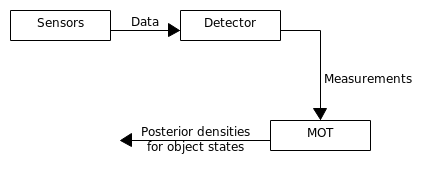
\includegraphics[scale=0.480]{img/object_tracking/sensor_mot_block_diagram.png}
\end{center}
\caption{MOT block diagram.}
\label{sensor_mot_block_diagram}
\end{figure}

\begin{figure}[!htb]
\begin{center}
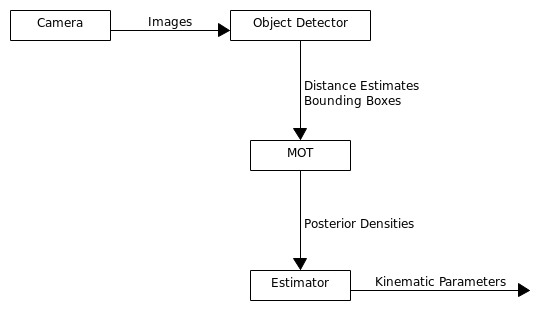
\includegraphics[scale=0.480]{img/object_tracking/camera_block_diagram.png}
\end{center}
\caption{Camera block diagram.}
\label{camera_block_diagram}
\end{figure}


\subsection{Challenges in MOT}
\label{challenges_mot}

Despite the abudance of the different MOT methodologies, problems do arise. In this section we will outline some of the problems
and challenges that typically an engineer, or whoever is atsked with developing a MOT pipeline whatsoever, has to face.

Let's consider again autonomous vehicle driving along a road.  Assumme that the vehicle is equipped with a sensor. 
The first problem one is faced with, is the unknown number of objects in the sensor's FoV. In addition to this, we typically do not
know the state of these objects; where they are located, where they are going etc. Arguably, however, it may be possible to 
have a reasonable estimate of these state. Furthermore, the tracked objects may move around with their own speed and orientation. This results
in some objects leaving the FoV of the sensor whilst others, not tracted previously, enter the sensor's FoV.

\begin{framed}
\begin{remark}{}

In the relevant literature of target tracking, object appearance is sometimes called bilrth, while object disappearance
is often called death. 
\end{remark}
\end{framed}

Another problem frequently encountered in practice is that some objects may occlude others. Finally, sensors are not perfrect. Therefore, one
has to deal with the following two types of errors

\begin{itemize}
\item Missed detections
\item False detections
\end{itemize}

\subsection{Questions}

\begin{enumerate}
\item Which property or properties hold(s) for the track-before-detect method?
\item Which property or properties hold(s) for the point object tracking method?
\item Which property or properties hold(s) for the extended object tracking method?
\item Which property or properties hold(s) for the group object tracking method?
\item Which property or properties hold(s) for the tracking with multi-path propagation method?
\item Which property or properties hold(s) for the tracking with unresolved measurements method?
\item Which of the following challenges are added when considering Multiple Object?
\begin{enumerate}
\item An unknown and time-varying number of objects
\item The state of each object is unknown and changes over time. 
\item The object states cannot be fully observed directly, have to be inferred from partial measurements.
\item The measurements are corrupted by noise, and are susceptible to missed detections and false detections. 
\item An unknown correspondence between multi-objects and their corresponding object-originated measurements. 
\end{enumerate}
\end{enumerate}

\subsection{Assignements}

\clearpage
\input{intro_answers.tex}
\clearpage
\bibliographystyle{plain}
\input{references.bbl}

\end{document}
